\documentclass[aspectratio=169,10pt]{beamer}

\usetheme{Madrid}
\usecolortheme{seahorse}

\usepackage{amsmath,amssymb,amsfonts}
\usepackage{bm}
\usepackage{graphicx}
\usepackage{listings}
\usepackage{xcolor}
\usepackage{booktabs}
\usepackage{tikz}
\usepackage{mathtools}

\graphicspath{{figures/}}

\setbeamertemplate{footline}[frame number]
\setbeamertemplate{navigation symbols}{}

% ── listing style ─────────────────────────────────────────────────────────────
\lstset{
  language=Python,
  basicstyle=\ttfamily\scriptsize,
  numbers=left,
  numberstyle=\tiny\color{gray},
  frame=single,
  backgroundcolor=\color{gray!7},
  keywordstyle=\color{blue!80!black}\bfseries,
  stringstyle=\color{red!60!black},
  commentstyle=\color{green!50!black}\itshape,
  showstringspaces=false,
  breaklines=true,
  tabsize=4,
}

% ── convenience macros ────────────────────────────────────────────────────────
\newcommand{\bx}{\mathbf{x}}
\newcommand{\by}{\mathbf{y}}
\newcommand{\bmu}{\boldsymbol{\mu}}
\newcommand{\bSigma}{\boldsymbol{\Sigma}}
\newcommand{\Real}{\mathbb{R}}
\newcommand{\Norm}{\mathcal{N}}
\newcommand{\GP}{\mathcal{GP}}
\newcommand{\KXX}{\mathbf{K}(X,X)}
\newcommand{\KXs}{\mathbf{K}(X^*,X)}
\newcommand{\KsX}{\mathbf{K}(X,X^*)}
\newcommand{\Kss}{\mathbf{K}(X^*,X^*)}

% ── title page ────────────────────────────────────────────────────────────────
\title[Ch.\ 18: Probabilistic Surrogate Models]{%
  Chapter 18: Probabilistic Surrogate Models}
\subtitle{Algorithms for Optimization, 2nd Edition (2026)\\
  Kochenderfer \& Wheeler}
\author{Lecture Slides}
\date{\today}

% ══════════════════════════════════════════════════════════════════════════════
\begin{document}
% ══════════════════════════════════════════════════════════════════════════════

\begin{frame}
  \titlepage
\end{frame}

%──────────────────────────────────────────────────────────────────────────────
\begin{frame}{Chapter Overview}
  \tableofcontents
\end{frame}

% ══════════════════════════════════════════════════════════════════════════════
\section{Motivation}
% ══════════════════════════════════════════════════════════════════════════════

\begin{frame}{Why Probabilistic Surrogate Models?}
  \begin{columns}[T]
    \begin{column}{0.55\textwidth}
      \begin{block}{Key Idea}
        When optimizing expensive black-box functions, we want not just a
        \emph{prediction} but also a measure of \emph{confidence}.
      \end{block}
      \vspace{0.4em}
      \begin{itemize}
        \item Deterministic surrogates (polynomial, RBF) give predictions
              but no uncertainty quantification.
        \item \textbf{Gaussian processes (GPs)} represent a probability
              distribution over functions.
        \item A GP posterior gives a \textbf{mean prediction} and a
              \textbf{variance} at every query point.
        \item Uncertainty can drive intelligent exploration (Bayesian
              optimization, Chapter 19).
      \end{itemize}
    \end{column}
    \begin{column}{0.42\textwidth}
      \begin{figure}
        \centering
        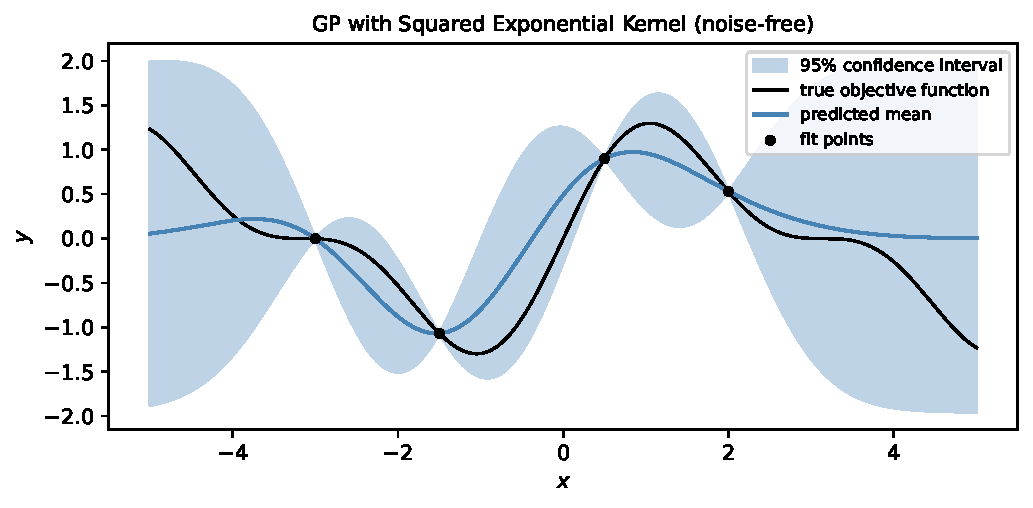
\includegraphics[width=\textwidth]{fig_gp_prediction.pdf}
        \caption{GP posterior mean and 95\% confidence interval fitted to
                 four noise-free evaluations.}
      \end{figure}
    \end{column}
  \end{columns}
\end{frame}

% ══════════════════════════════════════════════════════════════════════════════
\section{18.1 Gaussian Distribution}
% ══════════════════════════════════════════════════════════════════════════════

\begin{frame}{18.1 Multivariate Gaussian Distribution}
  \begin{columns}[T]
    \begin{column}{0.52\textwidth}
      \begin{block}{Definition (Eq.\ 18.1)}
        An $n$-dimensional \textbf{Gaussian distribution} is parametrised by
        mean $\bmu \in \Real^n$ and positive semi-definite covariance matrix
        $\bSigma \in \Real^{n\times n}$:
        \[
          \Norm(\bx\mid\bmu,\bSigma)
          = (2\pi)^{-n/2}|\bSigma|^{-1/2}
            \exp\!\Bigl(-\tfrac{1}{2}(\bx-\bmu)^\top\bSigma^{-1}(\bx-\bmu)\Bigr)
        \]
      \end{block}
      We write $\bx \sim \Norm(\bmu,\bSigma)$.\\[0.5em]
      \textbf{Covariance matrix structure:}
      \begin{itemize}
        \item Diagonal $\Sigma_{ii}$: variance of each component
        \item Off-diagonal $\Sigma_{ij}$: covariance between components $i,j$
        \item $\bSigma$ must be positive semi-definite
      \end{itemize}
    \end{column}
    \begin{column}{0.45\textwidth}
      \begin{figure}
        \centering
        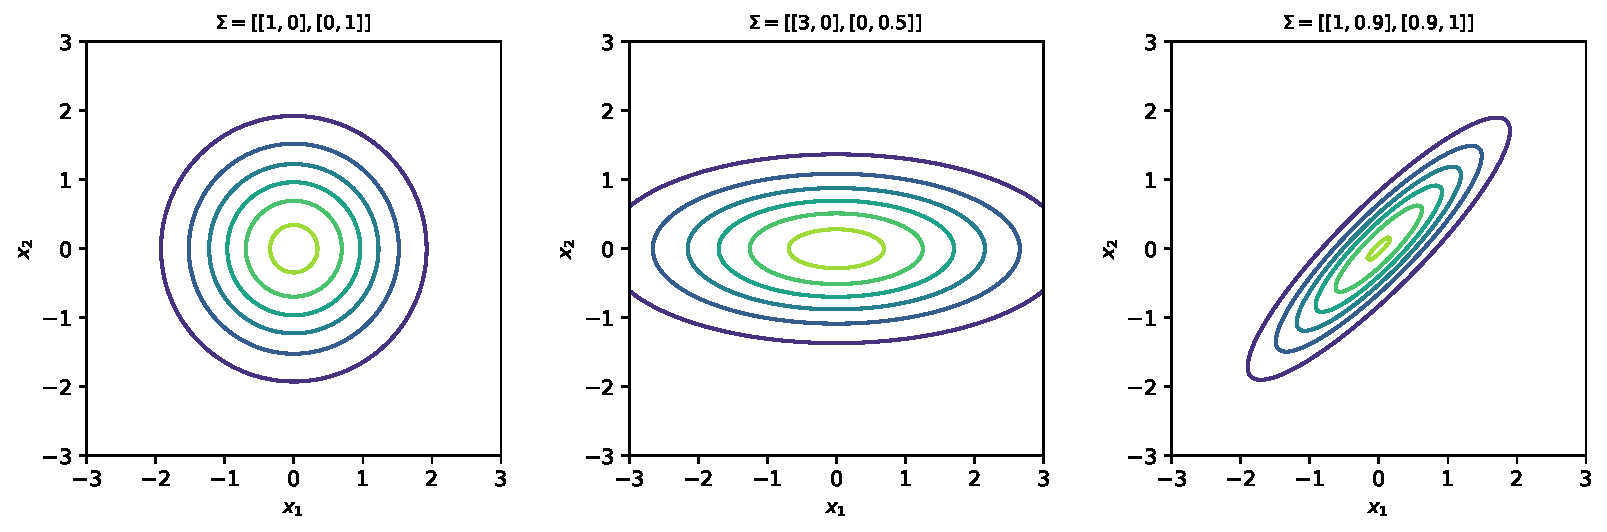
\includegraphics[width=\textwidth]{fig_gaussian_contours.pdf}
        \caption{Contour plots of 2D Gaussians with different $\bSigma$: identity
                 (circular), diagonal (ellipse), and correlated.}
      \end{figure}
    \end{column}
  \end{columns}
\end{frame}

\begin{frame}{Joint, Marginal, and Conditional Gaussians}
  \begin{block}{Joint distribution (Eq.\ 18.3)}
    Two jointly Gaussian random variables $\mathbf{a}$ and $\mathbf{b}$:
    \[
      \begin{bmatrix}\mathbf{a}\\\mathbf{b}\end{bmatrix}
      \sim \Norm\!\left(
        \begin{bmatrix}\bmu_a\\\bmu_b\end{bmatrix},\,
        \begin{bmatrix}\mathbf{A} & \mathbf{C}\\\mathbf{C}^\top & \mathbf{B}\end{bmatrix}
      \right)
    \]
  \end{block}
  \vspace{0.2em}
  \begin{columns}[T]
    \begin{column}{0.48\textwidth}
      \begin{block}{Marginal distributions (Eq.\ 18.4)}
        \[
          \mathbf{a}\sim\Norm(\bmu_a,\mathbf{A}),\quad
          \mathbf{b}\sim\Norm(\bmu_b,\mathbf{B})
        \]
        \emph{Sum out} the other variable.
      \end{block}
    \end{column}
    \begin{column}{0.48\textwidth}
      \begin{block}{Conditional distribution (Eqs.\ 18.5--18.7)}
        \[
          \mathbf{a}\mid\mathbf{b}
          \sim \Norm(\bmu_{a|b},\,\bSigma_{a|b})
        \]
        \[
          \bmu_{a|b}   = \bmu_a + \mathbf{C}\mathbf{B}^{-1}(\mathbf{b}-\bmu_b)
        \]
        \[
          \bSigma_{a|b} = \mathbf{A} - \mathbf{C}\mathbf{B}^{-1}\mathbf{C}^\top
        \]
      \end{block}
    \end{column}
  \end{columns}
  \vspace{0.3em}
  \begin{alertblock}{Key fact}
    Both the marginal and conditional distributions of a multivariate Gaussian
    are themselves Gaussian --- an extremely convenient closed-form property.
  \end{alertblock}
\end{frame}

\begin{frame}{Conditional Gaussian -- Numerical Example (Ex.\ 18.1)}
  \begin{columns}[T]
    \begin{column}{0.50\textwidth}
      \textbf{Setup:} Joint distribution over $(x_1, x_2)$:
      \[
        \begin{bmatrix}x_1\\x_2\end{bmatrix}
        \sim \Norm\!\left(
          \begin{bmatrix}0\\0\end{bmatrix},\,
          \begin{bmatrix}2 & 1\\1 & 1.5\end{bmatrix}
        \right)
      \]
      \vspace{0.3em}
      \textbf{Marginals:}
      \[
        x_1 \sim \Norm(0, 2), \quad x_2 \sim \Norm(0, 1.5)
      \]
      \vspace{0.3em}
      \textbf{Conditional} $x_1 \mid x_2 = 1$:
      \begin{align*}
        \mu_{1|2} &= 0 + \frac{1}{1.5}(1-0) = \tfrac{2}{3}\\
        \sigma^2_{1|2} &= 2 - \frac{1^2}{1.5} = \tfrac{4}{3}
      \end{align*}
    \end{column}
    \begin{column}{0.48\textwidth}
      \begin{figure}
        \centering
        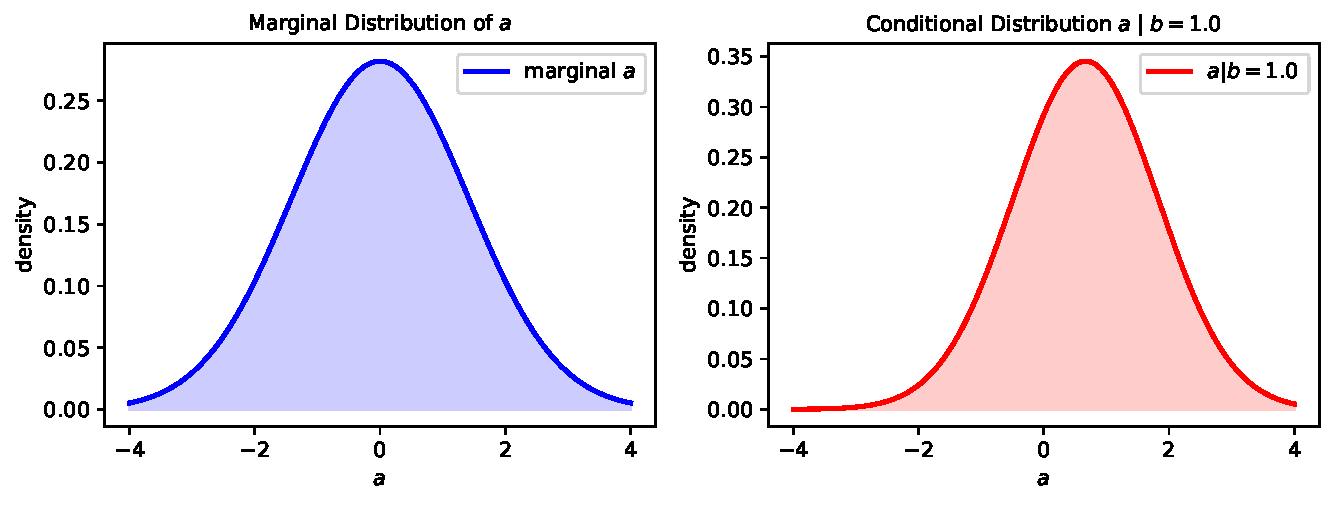
\includegraphics[width=\textwidth]{fig_conditional_gaussian.pdf}
        \caption{Marginal distribution of $x_1$ (left) vs.\ conditional
                 distribution $x_1\mid x_2=1$ (right). Conditioning
                 shifts the mean and reduces variance.}
      \end{figure}
    \end{column}
  \end{columns}
\end{frame}

% ══════════════════════════════════════════════════════════════════════════════
\section{18.2 Gaussian Processes}
% ══════════════════════════════════════════════════════════════════════════════

\begin{frame}{18.2 Gaussian Processes}
  \begin{block}{Definition}
    A \textbf{Gaussian process} $\GP(m, k)$ is a probability distribution over
    \emph{functions} $f : \Real^n \to \Real$.
    \begin{itemize}
      \item \textbf{Mean function} $m(\bx) = \mathbb{E}[f(\bx)]$
            (often zero)
      \item \textbf{Covariance/kernel function} $k(\bx,\bx') =
            \mathrm{Cov}(f(\bx),f(\bx'))$
    \end{itemize}
  \end{block}
  \vspace{0.3em}
  \begin{columns}[T]
    \begin{column}{0.48\textwidth}
      \textbf{Finite-dimensional view:}  For any finite set of points
      $X = \{\bx^{(1)},\ldots,\bx^{(m)}\}$, the values
      $[f(\bx^{(1)}),\ldots,f(\bx^{(m)})]^\top$ follow a multivariate
      Gaussian:
      \[
        \mathbf{y} \sim \Norm\bigl(\mathbf{m}(X),\,\mathbf{K}(X,X)\bigr)
      \]
      where $[\mathbf{K}(X,X)]_{ij} = k(\bx^{(i)},\bx^{(j)})$.
    \end{column}
    \begin{column}{0.48\textwidth}
      \textbf{Properties:}
      \begin{itemize}
        \item Nonparametric: complexity grows with data
        \item Fully determined by $m$ and $k$
        \item Analytically tractable posterior
        \item Computational cost $O(m^3)$ (matrix inversion)
      \end{itemize}
    \end{column}
  \end{columns}
\end{frame}

\begin{frame}{Kernel (Covariance) Functions}
  The kernel $k(\bx, \bx')$ encodes our prior belief about function smoothness.
  \vspace{0.5em}
  \begin{columns}[T]
    \begin{column}{0.52\textwidth}
      \renewcommand{\arraystretch}{1.5}
      \begin{tabular}{ll}
        \toprule
        \textbf{Kernel} & \textbf{Formula} \\
        \midrule
        Constant        & $c_f^2$ \\
        Linear          & $\sum_d c_d^2 x_d x_d'$ \\
        Polynomial      & $(x^\top x' + c_p^2)^p$ \\
        Exponential     & $\exp(-r)$ \\
        $\gamma$-Exponential & $\exp(-(r/\ell)^\gamma)$ \\
        Squared Exp.    & $\exp\!\left(-\dfrac{r^2}{2\ell^2}\right)$ \\
        Mat\'{e}rn      & $\frac{2^{1-\nu}}{\Gamma(\nu)}\bigl(\tfrac{\sqrt{2\nu}}{\ell}r\bigr)^\nu
                          K_\nu\bigl(\tfrac{\sqrt{2\nu}}{\ell}r\bigr)$ \\
        Rat.\ Quadratic & $\left(1+\dfrac{r^2}{2\alpha\ell^2}\right)^{-\alpha}$ \\
        \bottomrule
      \end{tabular}
      \vspace{0.3em}
      {\footnotesize $r = \|\bx-\bx'\|$}
    \end{column}
    \begin{column}{0.45\textwidth}
      \begin{figure}
        \centering
        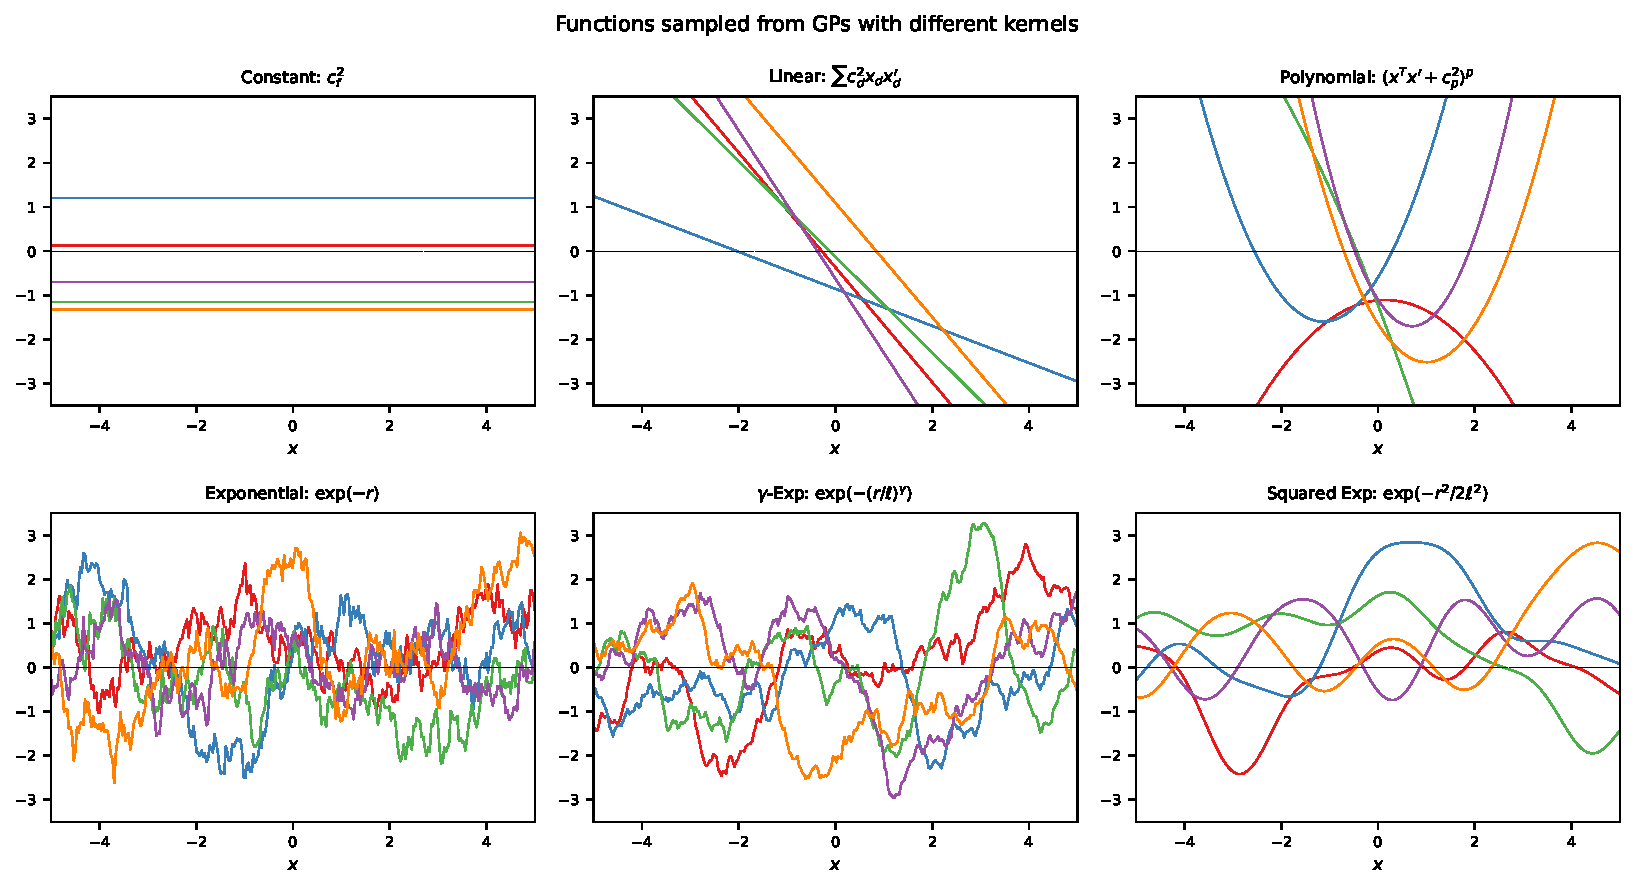
\includegraphics[width=\textwidth]{fig_kernel_samples.pdf}
        \caption{Functions sampled from GPs with different kernels.
                 Smoother kernels produce smoother sample paths.}
      \end{figure}
    \end{column}
  \end{columns}
\end{frame}

\begin{frame}[fragile]{Kernel Functions in Python}
\begin{lstlisting}
import numpy as np

def sq_exp_kernel(x1, x2, ell=1.0, sigma_f=1.0):
    """Squared exponential (RBF) kernel."""
    r2 = np.sum((x1 - x2)**2)
    return sigma_f**2 * np.exp(-r2 / (2 * ell**2))

def matern52_kernel(x1, x2, ell=1.0):
    """Matern 5/2 kernel."""
    r = np.sqrt(np.sum((x1 - x2)**2))
    t = np.sqrt(5) * r / ell
    return (1 + t + t**2 / 3) * np.exp(-t)

def rat_quad_kernel(x1, x2, ell=1.0, alpha=1.0):
    """Rational quadratic kernel."""
    r2 = np.sum((x1 - x2)**2)
    return (1 + r2 / (2 * alpha * ell**2))**(-alpha)

# Build kernel matrix K(X, X)
def build_K(X, kernel, noise=0.0):
    m = len(X)
    K = np.array([[kernel(X[i], X[j]) for j in range(m)]
                  for i in range(m)])
    return K + (noise + 1e-8) * np.eye(m)
\end{lstlisting}
\end{frame}

\begin{frame}{Key Property: Squared Exponential Kernel}
  \begin{columns}[T]
    \begin{column}{0.50\textwidth}
      \begin{block}{Squared Exponential (SE) kernel}
        \[
          k(\bx, \bx') = \exp\!\left(-\frac{\|\bx - \bx'\|^2}{2\ell^2}\right)
        \]
        \begin{itemize}
          \item $\ell$: \textbf{length-scale} (horizontal scale)
          \item Corresponds to smooth ($C^\infty$) functions
          \item \textbf{Stationarity}: depends only on $\bx - \bx'$
          \item $k(\bx,\bx) = 1$ (unit variance prior)
        \end{itemize}
      \end{block}
      \vspace{0.3em}
      \textbf{Interpretation:} Two points close together
      ($\|\bx-\bx'\| \ll \ell$) are highly correlated; far-apart points
      ($\|\bx-\bx'\| \gg \ell$) are nearly independent.
    \end{column}
    \begin{column}{0.47\textwidth}
      \begin{figure}
        \centering
        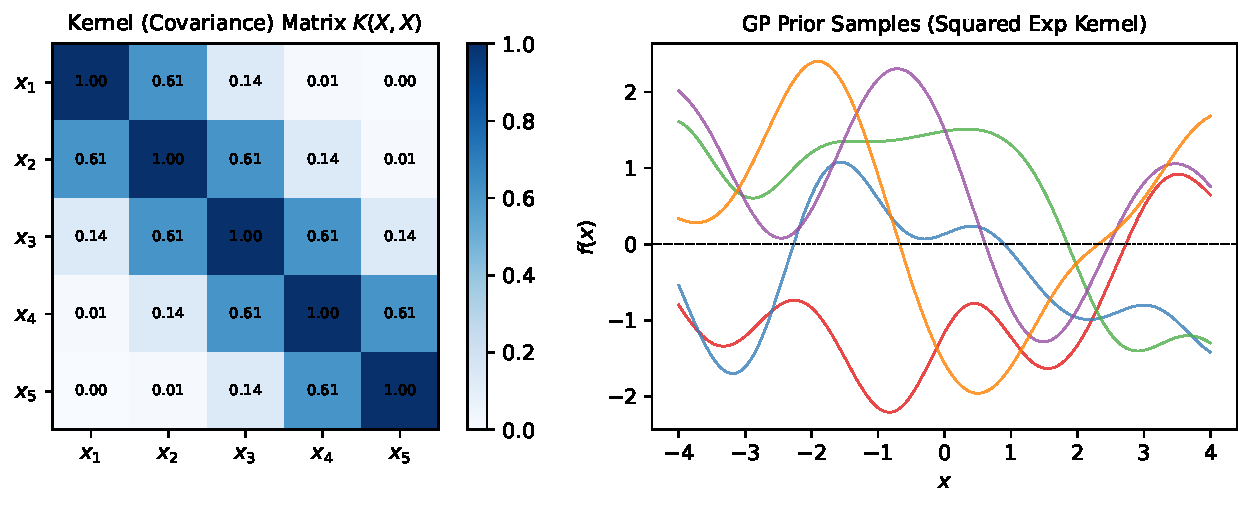
\includegraphics[width=\textwidth]{fig_kernel_matrix.pdf}
        \caption{Kernel (covariance) matrix for 5 equally-spaced points
                 (left) and GP prior samples (right).}
      \end{figure}
    \end{column}
  \end{columns}
\end{frame}

% ══════════════════════════════════════════════════════════════════════════════
\section{18.3 Prediction (Posterior Mean and Variance)}
% ══════════════════════════════════════════════════════════════════════════════

\begin{frame}{18.3 GP Prediction -- Setup}
  \begin{block}{Given}
    \begin{itemize}
      \item Training data: $m$ observations $(X, \mathbf{y})$ where
            $X = \{\bx^{(1)},\ldots,\bx^{(m)}\}$ and
            $\mathbf{y} = [y^{(1)},\ldots,y^{(m)}]^\top$
      \item Query (test) points: $X^*$ ($\ell$ points)
      \item GP prior: $\GP(m(\cdot), k(\cdot,\cdot))$
    \end{itemize}
  \end{block}
  \vspace{0.3em}
  \textbf{Joint prior distribution} (Eq.\ 18.10):
  \[
    \begin{bmatrix}\hat{\mathbf{y}}\\\mathbf{y}\end{bmatrix}
    \sim \Norm\!\left(
      \begin{bmatrix}\mathbf{m}(X^*)\\\mathbf{m}(X)\end{bmatrix},\,
      \begin{bmatrix}
        \mathbf{K}(X^*,X^*) & \mathbf{K}(X^*,X) \\
        \mathbf{K}(X,X^*)   & \mathbf{K}(X,X)
      \end{bmatrix}
    \right)
  \]
  \vspace{0.3em}
  Apply the conditional Gaussian formula (Eqs.\ 18.5--18.7) to obtain the
  \textbf{posterior} $\hat{\mathbf{y}} \mid \mathbf{y}$.
\end{frame}

\begin{frame}{18.3 GP Posterior (Noise-Free)}
  \begin{block}{Posterior distribution (Eqs.\ 18.13--18.16)}
    \[
      \hat{\mathbf{y}} \mid \mathbf{y}
      \;\sim\; \Norm\!\bigl(\hat{\bmu},\, \hat{\bSigma}\bigr)
    \]
    \[
      \hat{\bmu}    = \mathbf{m}(X^*) +
                      \KXs^\top \KXX^{-1}\bigl(\mathbf{y}-\mathbf{m}(X)\bigr)
    \]
    \[
      \hat{\bSigma} = \Kss - \KXs^\top \KXX^{-1} \KXs
    \]
  \end{block}
  \vspace{0.2em}
  \begin{columns}[T]
    \begin{column}{0.46\textwidth}
      \textbf{Symbol guide:}
      \begin{itemize}
        \item $\mathbf{K}(X^*,X)$: $\ell\times m$ cross-covariance matrix
        \item $\mathbf{K}(X,X)$: $m\times m$ training covariance matrix
        \item $\mathbf{K}(X^*,X^*)$: $\ell\times\ell$ test covariance matrix
        \item Posterior is also referred to as the \emph{posterior distribution}
      \end{itemize}
      \vspace{0.3em}
      \textbf{Predictive variance} at a single point $\bx^*$:
      \[
        \hat{v}(\bx^*) = k(\bx^*,\bx^*) - \mathbf{k}_{*}^\top \KXX^{-1} \mathbf{k}_{*}
      \]
    \end{column}
    \begin{column}{0.50\textwidth}
      \textbf{Complexity:}
      \begin{itemize}
        \item Matrix inversion $\KXX^{-1}$: $O(m^3)$
        \item Prediction at $\ell$ points: $O(m^2 \ell)$
        \item Bottleneck: $m^3$ grows fast --- sparse/approximate GP methods
              address this at scale
      \end{itemize}
      \vspace{0.3em}
      \textbf{95\% confidence region} (Eq.\ 18.17):
      \[
        \hat{\mu}(\bx) \pm 1.96\,\hat{\sigma}(\bx)
      \]
      where $\hat{\sigma}(\bx)=\sqrt{\hat{v}(\bx)}$.
    \end{column}
  \end{columns}
\end{frame}

\begin{frame}[fragile]{GP Prediction in Python (Algorithm 18.2)}
\begin{lstlisting}
import numpy as np

def gp_predict(X_train, y_train, X_pred, kernel, noise=0.0):
    """
    Gaussian process prediction.
    Returns posterior mean mu and variance var at X_pred.
    """
    m = len(X_train)
    n = len(X_pred)

    # Build covariance matrices
    K_XX = np.array([[kernel(X_train[i], X_train[j])
                      for j in range(m)] for i in range(m)])
    K_XX += (noise + 1e-8) * np.eye(m)          # regularise

    K_Xs = np.array([[kernel(X_pred[i], X_train[j])
                      for j in range(m)] for i in range(n)])

    K_ss = np.array([[kernel(X_pred[i], X_pred[j])
                      for j in range(n)] for i in range(n)])

    # Posterior
    K_inv = np.linalg.solve(K_XX, np.eye(m))     # O(m^3)
    mu    = K_Xs @ K_inv @ y_train               # posterior mean
    cov   = K_ss - K_Xs @ K_inv @ K_Xs.T        # posterior covariance
    var   = np.diag(cov)                          # marginal variances

    return mu, np.maximum(var, 0)
\end{lstlisting}
\end{frame}

\begin{frame}{GP Prediction -- Numerical Example}
  \begin{columns}[T]
    \begin{column}{0.50\textwidth}
      \textbf{Setup:}
      \begin{itemize}
        \item Kernel: SE with $\ell = 1$, $\sigma_f = 1$
        \item Training points: $x \in \{-3, -1.5, 0.5, 2.0\}$
        \item True function: $f(x) = \sin(x) + 0.5\sin(2x)$
        \item Zero mean GP prior
      \end{itemize}
      \vspace{0.4em}
      \textbf{Observations:}
      \begin{itemize}
        \item Posterior mean interpolates training data exactly
        \item Uncertainty (shaded region) is small near training points
        \item Uncertainty grows far from training data
        \item Expected value $\to 0$ as $x \to \pm\infty$
      \end{itemize}
    \end{column}
    \begin{column}{0.47\textwidth}
      \begin{figure}
        \centering
        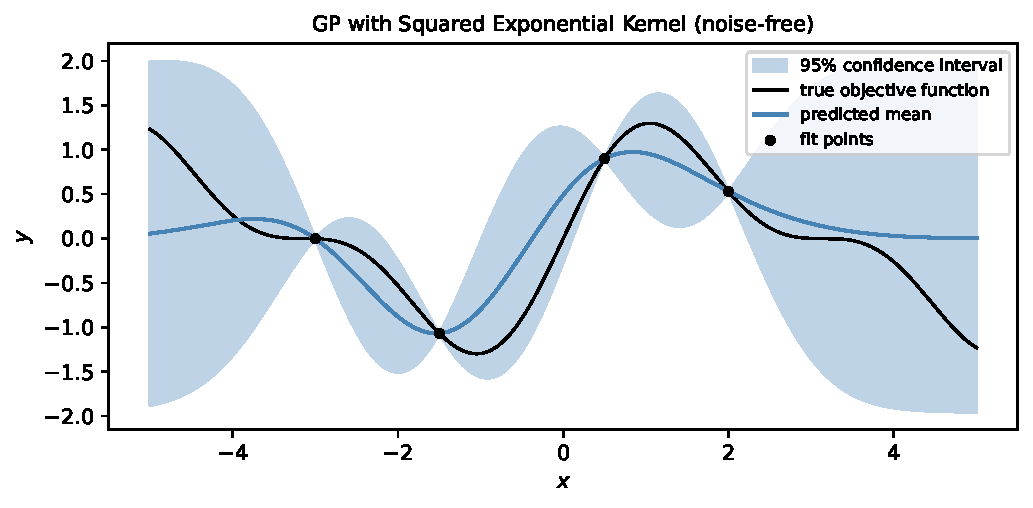
\includegraphics[width=\textwidth]{fig_gp_prediction.pdf}
        \caption{GP posterior with 95\% confidence interval.}
      \end{figure}
    \end{column}
  \end{columns}
\end{frame}

\begin{frame}{2D Gaussian Process}
  \begin{columns}[T]
    \begin{column}{0.48\textwidth}
      GPs naturally extend to multi-dimensional design spaces.
      \vspace{0.5em}
      \begin{itemize}
        \item Same formulas apply; $\bx \in \Real^n$
        \item Kernel $k(\bx,\bx')$ must be positive semi-definite
        \item SE kernel: $k(\bx,\bx')=\exp\!\bigl(-\frac{1}{2\ell^2}\|\bx-\bx'\|^2\bigr)$
        \item Cost scales as $O(m^3)$ regardless of $n$
      \end{itemize}
      \vspace{0.5em}
      \textbf{Note:} Covariance matrix size is $m\times m$ (number of
      observations), \emph{not} related to input dimension $n$.
    \end{column}
    \begin{column}{0.49\textwidth}
      \begin{figure}
        \centering
        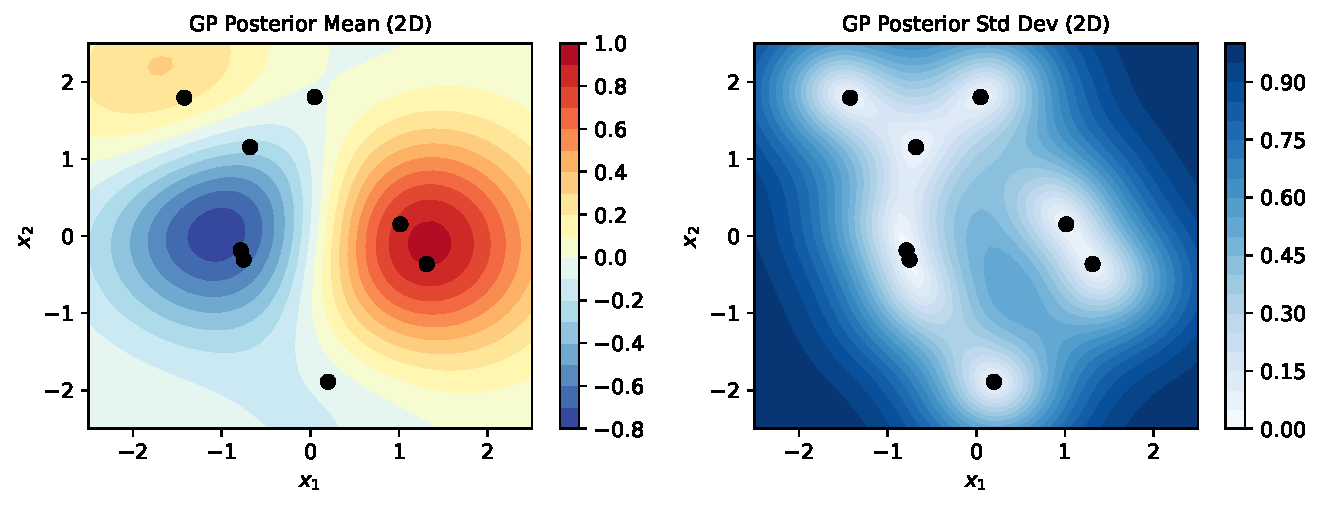
\includegraphics[width=\textwidth]{fig_gp_2d.pdf}
        \caption{GP posterior mean (left) and standard deviation (right)
                 fitted to 8 random observations in 2D. Black dots mark
                 training points.}
      \end{figure}
    \end{column}
  \end{columns}
\end{frame}

% ══════════════════════════════════════════════════════════════════════════════
\section{18.4 Gradient Measurements}
% ══════════════════════════════════════════════════════════════════════════════

\begin{frame}{18.4 Gradient Measurements -- Motivation}
  \begin{columns}[T]
    \begin{column}{0.55\textwidth}
      \begin{block}{Key insight}
        Gradient information is \emph{free} in many applications
        (automatic differentiation, adjoint methods).
        Each gradient observation adds $n$ constraints, significantly
        reducing uncertainty.
      \end{block}
      \vspace{0.3em}
      \textbf{Extended GP model (Eq.\ 18.18):}
      \[
        \begin{bmatrix}\mathbf{y}\\\nabla\mathbf{y}\end{bmatrix}
        \sim \Norm\!\left(
          \begin{bmatrix}\mathbf{m}_f\\\mathbf{m}_\nabla\end{bmatrix},\,
          \begin{bmatrix}
            \mathbf{K}_{ff} & \mathbf{K}_{f\nabla}\\
            \mathbf{K}_{\nabla f} & \mathbf{K}_{\nabla\nabla}
          \end{bmatrix}
        \right)
      \]
      \vspace{0.2em}
      where each covariance block is derived from the base kernel $k$.
    \end{column}
    \begin{column}{0.42\textwidth}
      \begin{figure}
        \centering
        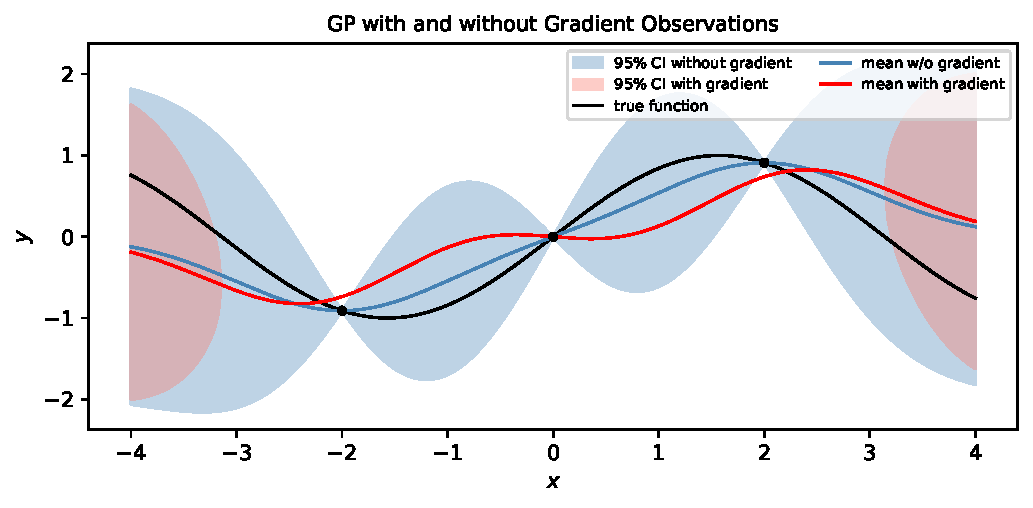
\includegraphics[width=\textwidth]{fig_gp_gradient.pdf}
        \caption{GP with (salmon) and without (blue) gradient observations.
                 Gradient information significantly tightens the
                 confidence interval.}
      \end{figure}
    \end{column}
  \end{columns}
\end{frame}

\begin{frame}{Covariance Functions with Gradients (Eqs.\ 18.19--18.22)}
  \begin{block}{Derived covariance functions (via linearity of covariance)}
    \[
      k_{ff}(\bx,\bx') = k(\bx,\bx') \qquad\text{(original kernel)}
    \]
    \[
      k_{\nabla f}(\bx,\bx')_i = \nabla_{\bx_i} k(\bx,\bx')
    \]
    \[
      k_{f\nabla}(\bx,\bx')_i = \nabla_{\bx'_i} k(\bx,\bx')
    \]
    \[
      k_{\nabla\nabla}(\bx,\bx')_{ij} = \nabla_{\bx_i}\nabla_{\bx'_j} k(\bx,\bx')
    \]
  \end{block}
  \vspace{0.3em}
  \begin{block}{Example 18.2: SE kernel derivatives}
    For $k_{ff}(\bx,\bx') = \exp\bigl(-\tfrac{1}{2}\|\bx-\bx'\|^2\bigr)$:
    \begin{align*}
      k_{\nabla f}(\bx,\bx')_i &= -(x_i - x'_i)\exp\bigl(-\tfrac{1}{2}\|\bx-\bx'\|^2\bigr)\\
      k_{\nabla\nabla}(\bx,\bx')_{ij} &= -\bigl((i=j) - (x_i-x'_i)(x_j-x'_j)\bigr)
                                          \exp\bigl(-\tfrac{1}{2}\|\bx-\bx'\|^2\bigr)
    \end{align*}
    where $(i=j)$ evaluates to 1 if true, 0 if false.
  \end{block}
\end{frame}

\begin{frame}{GP Posterior with Gradients (Eqs.\ 18.25--18.27)}
  \textbf{Joint distribution for prediction} (Eq.\ 18.23):
  \[
    \begin{bmatrix}\hat{\mathbf{y}}\\\mathbf{y}\\\nabla\mathbf{y}\end{bmatrix}
    \sim \Norm\!\left(
      \begin{bmatrix}\mathbf{m}_f(X^*)\\\mathbf{m}_f(X)\\\mathbf{m}_\nabla(X)\end{bmatrix},\,
      \begin{bmatrix}
        \mathbf{K}_{ff}(X^*,X^*) & \mathbf{K}_{ff}(X^*,X) & \mathbf{K}_{f\nabla}(X^*,X)\\
        \mathbf{K}_{ff}(X,X^*)   & \mathbf{K}_{ff}(X,X)   & \mathbf{K}_{f\nabla}(X,X)\\
        \mathbf{K}_{\nabla f}(X,X^*)& \mathbf{K}_{\nabla f}(X,X) & \mathbf{K}_{\nabla\nabla}(X,X)
      \end{bmatrix}
    \right)
  \]
  \vspace{0.2em}
  \begin{block}{Posterior (same formula as before, Eqs.\ 18.25--18.27)}
    \[
      \hat{\mathbf{y}}\mid\mathbf{y},\nabla\mathbf{y}
      \sim \Norm(\bmu_\nabla, \bSigma_\nabla)
    \]
    \[
      \bmu_\nabla = \mathbf{m}_f(X^*) +
        \begin{bmatrix}\mathbf{K}_{ff}(X^*,X)\\\mathbf{K}_{\nabla f}(X^*,X)\end{bmatrix}^\top
        \begin{bmatrix}\mathbf{K}_{ff}(X,X) & \mathbf{K}_{f\nabla}(X,X)\\
                       \mathbf{K}_{\nabla f}(X,X) & \mathbf{K}_{\nabla\nabla}(X,X)\end{bmatrix}^{-1}
        \begin{bmatrix}\mathbf{y}-\mathbf{m}_f(X)\\\nabla\mathbf{y}-\mathbf{m}_\nabla(X)\end{bmatrix}
    \]
  \end{block}
  \vspace{0.2em}
  \textbf{Covariance block dimensions} (Eq.\ 18.24):
  $\ell\times\ell$, $\ell\times m$, $\ell\times nm$, $m\times m$, $m\times nm$,
  $nm\times nm$ where $\ell$ = query pts, $m$ = obs, $n$ = input dim.
\end{frame}

\begin{frame}[fragile]{Gradient GP in Python}
\begin{lstlisting}
import numpy as np

def kff(x, xp, ell=1.0):
    return np.exp(-0.5 * (x - xp)**2 / ell**2)

def kvf(x, xp, ell=1.0):   # d/dx k(x, xp)
    return -(x - xp) / ell**2 * kff(x, xp, ell)

def kvv(x, xp, ell=1.0):   # d^2/dx dx' k(x, xp)
    d = x - xp
    return (1.0/ell**2 - d**2/ell**4) * kff(x, xp, ell)

def gp_predict_with_gradients(X_obs, y_obs, dy_obs, X_pred, ell=1.0):
    m, n = len(X_obs), len(X_pred)
    # Build extended training covariance [K_ff K_fv; K_vf K_vv]
    K_ff = np.array([[kff(X_obs[i],X_obs[j],ell) for j in range(m)] for i in range(m)])
    K_vf = np.array([[kvf(X_obs[i],X_obs[j],ell) for j in range(m)] for i in range(m)])
    K_vv = np.array([[kvv(X_obs[i],X_obs[j],ell) for j in range(m)] for i in range(m)])
    K_tr = np.block([[K_ff, K_vf.T],[K_vf, K_vv]]) + 1e-8*np.eye(2*m)
    # Cross-covariances to prediction points
    Ksf  = np.array([[kff(X_pred[i],X_obs[j],ell) for j in range(m)] for i in range(n)])
    Ksv  = np.array([[kvf(X_pred[i],X_obs[j],ell) for j in range(m)] for i in range(n)])
    Ks   = np.hstack([Ksf, Ksv])
    # Posterior mean
    y_comb = np.concatenate([y_obs, dy_obs])
    mu = Ks @ np.linalg.solve(K_tr, y_comb)
    return mu
\end{lstlisting}
\end{frame}

% ══════════════════════════════════════════════════════════════════════════════
\section{18.5 Noisy Measurements}
% ══════════════════════════════════════════════════════════════════════════════

\begin{frame}{18.5 Noisy Measurements}
  \begin{columns}[T]
    \begin{column}{0.55\textwidth}
      \begin{block}{Model (Eq.\ 18.28)}
        Observations include zero-mean Gaussian noise:
        \[
          y = f(\bx) + z, \quad z \sim \Norm(0, \nu)
        \]
        \[
          \begin{bmatrix}\hat{\mathbf{y}}\\\mathbf{y}\end{bmatrix}
          \sim \Norm\!\left(
            \begin{bmatrix}\mathbf{m}(X^*)\\\mathbf{m}(X)\end{bmatrix},\,
            \begin{bmatrix}
              \mathbf{K}(X^*,X^*) & \mathbf{K}(X^*,X)\\
              \mathbf{K}(X,X^*)   & \mathbf{K}(X,X)+\nu\mathbf{I}
            \end{bmatrix}
          \right)
        \]
      \end{block}
      \vspace{0.3em}
      \textbf{Posterior (Eqs.\ 18.29--18.31):}
      \[
        \hat{\mathbf{y}}\mid\mathbf{y},\nu \sim \Norm(\bmu^*, \bSigma^*)
      \]
      \[
        \bmu^* = \mathbf{m}(X^*) + \mathbf{K}(X^*,X)\bigl(\mathbf{K}(X,X)+\nu\mathbf{I}\bigr)^{-1}
                 \bigl(\mathbf{y}-\mathbf{m}(X)\bigr)
      \]
      \[
        \bSigma^* = \mathbf{K}(X^*,X^*) - \mathbf{K}(X^*,X)
                    \bigl(\mathbf{K}(X,X)+\nu\mathbf{I}\bigr)^{-1}\mathbf{K}(X,X^*)
      \]
    \end{column}
    \begin{column}{0.42\textwidth}
      \begin{figure}
        \centering
        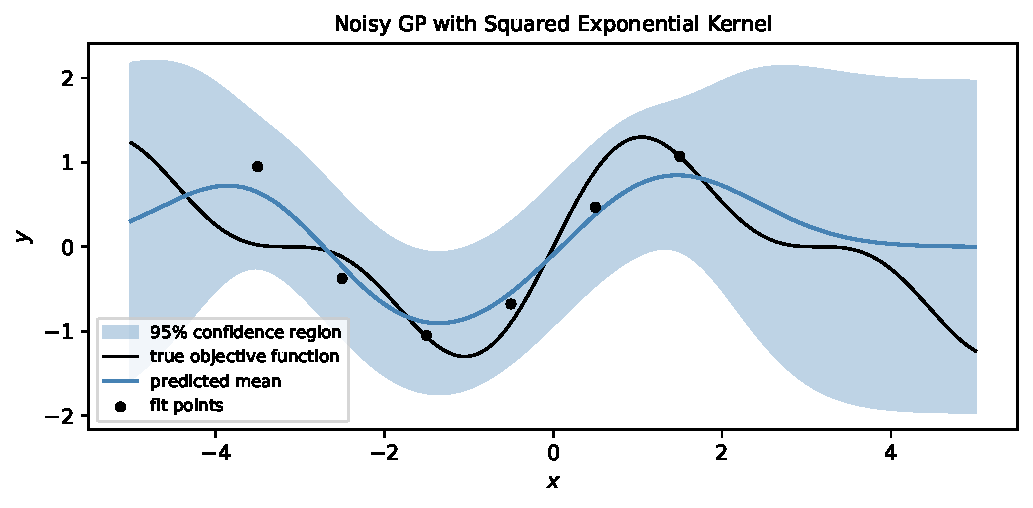
\includegraphics[width=\textwidth]{fig_gp_noisy.pdf}
        \caption{Noisy GP with SE kernel. The posterior does \emph{not}
                 exactly interpolate data; the noise $\nu$ controls the
                 balance between fit and smoothness.}
      \end{figure}
    \end{column}
  \end{columns}
\end{frame}

\begin{frame}[fragile]{Noisy GP Prediction in Python (Algorithm 18.4)}
\begin{lstlisting}
import numpy as np

def sq_exp_kernel(x1, x2, ell=1.0):
    return np.exp(-0.5 * (x1 - x2)**2 / ell**2)

def predict_noisy_gp(X_train, y_train, X_pred,
                     kernel, noise_var=0.1):
    """
    GP prediction with Gaussian observation noise.
    noise_var: variance nu of noise z ~ N(0, nu)
    Returns: mu_pred, var_pred
    """
    m = len(X_train)
    n = len(X_pred)

    K_XX = np.array([[kernel(X_train[i], X_train[j])
                      for j in range(m)] for i in range(m)])
    K_XX += (noise_var + 1e-8) * np.eye(m)   # add noise

    K_Xs = np.array([[kernel(X_pred[i], X_train[j])
                      for j in range(m)] for i in range(n)])
    K_ss_diag = np.array([kernel(X_pred[i], X_pred[i])
                           for i in range(n)])

    alpha  = np.linalg.solve(K_XX, y_train)
    mu     = K_Xs @ alpha
    tmp    = np.linalg.solve(K_XX, K_Xs.T)
    var    = K_ss_diag - np.sum(K_Xs * tmp.T, axis=1)

    return mu, np.maximum(var, 0)
\end{lstlisting}
\end{frame}

\begin{frame}{Noise-Free vs.\ Noisy GP: Key Differences}
  \begin{columns}[T]
    \begin{column}{0.48\textwidth}
      \textbf{Noise-free GP:}
      \begin{itemize}
        \item $\mathbf{K}(X,X) + \epsilon\mathbf{I}$ (small $\epsilon$ for numerical stability)
        \item Posterior \textbf{exactly interpolates} training data
        \item Posterior variance is zero at training points
        \item Appropriate when function evaluations are deterministic
      \end{itemize}
    \end{column}
    \begin{column}{0.48\textwidth}
      \textbf{Noisy GP:}
      \begin{itemize}
        \item $\mathbf{K}(X,X) + \nu\mathbf{I}$ (larger $\nu$ = more noise)
        \item Posterior \textbf{does not interpolate} --- smoothes through data
        \item Non-zero variance even at training points
        \item Appropriate for experimental data, simulation with randomness
        \item $\nu$ can be tuned via MLE (Section 18.6)
      \end{itemize}
    \end{column}
  \end{columns}
  \vspace{0.4em}
  \begin{alertblock}{Practical tip}
    Always add a small nugget term ($\epsilon \approx 10^{-8}$) for numerical
    stability when inverting the kernel matrix, even in the noise-free case.
  \end{alertblock}
\end{frame}

% ══════════════════════════════════════════════════════════════════════════════
\section{18.6 Fitting Gaussian Processes (MLE)}
% ══════════════════════════════════════════════════════════════════════════════

\begin{frame}{18.6 Fitting GP Hyperparameters via MLE}
  \begin{columns}[T]
    \begin{column}{0.55\textwidth}
      \begin{block}{Log marginal likelihood (Eq.\ 18.34)}
        GP parameters $\boldsymbol{\theta}$ (length-scale $\ell$, signal
        variance $\sigma_f^2$, noise $\nu$) are fitted by maximizing:
        \[
          \log p(\mathbf{y}\mid X,\boldsymbol{\theta})
          = -\tfrac{1}{2}\mathbf{y}^\top\mathbf{K}^{-1}\mathbf{y}
            -\tfrac{1}{2}\log|\mathbf{K}|
            -\tfrac{m}{2}\log 2\pi
        \]
        where $\mathbf{K} = \mathbf{K}(X,X;\boldsymbol{\theta}) + \nu\mathbf{I}$.
      \end{block}
      \vspace{0.3em}
      \textbf{Three terms:}
      \begin{enumerate}
        \item \textbf{Data fit}: $-\tfrac{1}{2}\mathbf{y}^\top\mathbf{K}^{-1}\mathbf{y}$
              --- rewards models that explain the data
        \item \textbf{Complexity penalty}: $-\tfrac{1}{2}\log|\mathbf{K}|$
              --- penalises overly flexible models (Occam's razor)
        \item \textbf{Normalisation}: constant
      \end{enumerate}
    \end{column}
    \begin{column}{0.42\textwidth}
      \begin{figure}
        \centering
        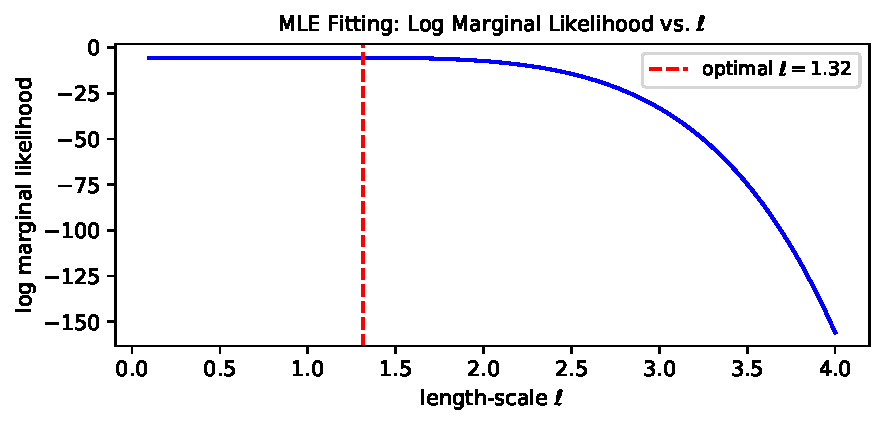
\includegraphics[width=\textwidth]{fig_mle_loglik.pdf}
        \caption{Log marginal likelihood as a function of the length-scale
                 $\ell$. The optimal $\ell$ balances fit and smoothness.}
      \end{figure}
    \end{column}
  \end{columns}
\end{frame}

\begin{frame}{Gradient of the Log Marginal Likelihood}
  \begin{block}{Gradient w.r.t.\ $\theta_j$ (Eq.\ 18.35)}
    \[
      \frac{\partial}{\partial\theta_j}\log p(\mathbf{y}\mid X,\boldsymbol{\theta})
      = \frac{1}{2}\mathbf{y}^\top\mathbf{K}^{-1}
        \frac{\partial\mathbf{K}}{\partial\theta_j}\mathbf{K}^{-1}\mathbf{y}
        - \frac{1}{2}\mathrm{tr}\!\left(\mathbf{K}^{-1}
          \frac{\partial\mathbf{K}}{\partial\theta_j}\right)
    \]
  \end{block}
  \vspace{0.3em}
  \begin{columns}[T]
    \begin{column}{0.52\textwidth}
      \textbf{Numerical considerations:}
      \begin{itemize}
        \item Use Cholesky decomposition for stability:
              $\mathbf{K} = \mathbf{L}\mathbf{L}^\top$
        \item $\log|\mathbf{K}| = 2\sum_i \log L_{ii}$
        \item $\mathbf{K}^{-1}\mathbf{y}$ via triangular solves
        \item Gradient enables gradient-based optimisation (L-BFGS-B)
        \item Multiple random restarts to avoid local optima
      \end{itemize}
    \end{column}
    \begin{column}{0.45\textwidth}
      \textbf{Typical hyperparameters:}\\[0.3em]
      \begin{tabular}{ll}
        \toprule
        \textbf{Parameter} & \textbf{Role}\\
        \midrule
        $\ell$ & length-scale (smoothness)\\
        $\sigma_f^2$ & signal variance (amplitude)\\
        $\nu$ & noise variance\\
        \bottomrule
      \end{tabular}\\[0.5em]
      Optimise in log-space to enforce positivity:
      $\theta_j = \exp(\tilde\theta_j)$.
    \end{column}
  \end{columns}
\end{frame}

\begin{frame}[fragile]{MLE Fitting in Python}
\begin{lstlisting}
import numpy as np
from scipy.optimize import minimize

def log_marginal_likelihood(params, X_train, y_train):
    log_ell, log_sf, log_nu = params
    ell = np.exp(log_ell); sf = np.exp(log_sf); nu = np.exp(log_nu)

    m = len(X_train)
    K = sf**2 * np.array([
        [np.exp(-0.5*((X_train[i]-X_train[j])/ell)**2)
         for j in range(m)] for i in range(m)])
    K += (nu + 1e-8) * np.eye(m)

    try:
        L = np.linalg.cholesky(K)
    except np.linalg.LinAlgError:
        return np.inf                        # non-PD: reject

    alpha   = np.linalg.solve(L.T, np.linalg.solve(L, y_train))
    log_det = 2.0 * np.sum(np.log(np.diag(L)))
    lml     = -0.5 * (y_train @ alpha + log_det
                      + m * np.log(2*np.pi))
    return -lml                              # negate for minimisation

# Optimise with multiple restarts
best = None
for _ in range(5):
    x0  = np.random.randn(3)               # random init in log-space
    res = minimize(log_marginal_likelihood, x0,
                   args=(X_train, y_train),
                   method='L-BFGS-B')
    if best is None or res.fun < best.fun:
        best = res
\end{lstlisting}
\end{frame}

% ══════════════════════════════════════════════════════════════════════════════
\section{Summary \& Exercises}
% ══════════════════════════════════════════════════════════════════════════════

\begin{frame}{Summary}
  \begin{columns}[T]
    \begin{column}{0.52\textwidth}
      \textbf{Key concepts:}
      \begin{enumerate}
        \item \textbf{Multivariate Gaussian} has closed-form marginal and
              conditional distributions --- the foundation of GPs.
        \item \textbf{Gaussian Process} = distribution over functions,
              characterised by mean $m(\bx)$ and kernel $k(\bx,\bx')$.
        \item \textbf{Kernel selection} determines smoothness; SE is the
              most common choice.
        \item \textbf{GP prediction}: posterior mean $\hat\bmu$ and covariance
              $\hat\bSigma$ via conditional Gaussian formula. Cost: $O(m^3)$.
        \item \textbf{Gradient measurements}: extend the GP using derivative
              kernel functions; significantly reduces uncertainty.
        \item \textbf{Noisy observations}: add $\nu\mathbf{I}$ to training
              covariance; posterior no longer interpolates.
        \item \textbf{MLE fitting}: maximise log marginal likelihood to learn
              kernel hyperparameters from data.
      \end{enumerate}
    \end{column}
    \begin{column}{0.45\textwidth}
      \textbf{Complexity summary:}\\[0.5em]
      \begin{tabular}{ll}
        \toprule
        \textbf{Operation} & \textbf{Cost}\\
        \midrule
        Build $\mathbf{K}(X,X)$ & $O(m^2)$\\
        Invert $\mathbf{K}(X,X)$ & $O(m^3)$\\
        Predict at $\ell$ points & $O(m^2\ell)$\\
        With gradients ($nm$ obs.) & $O((nm)^3)$\\
        MLE gradient & $O(m^3)$ per step\\
        \bottomrule
      \end{tabular}
      \vspace{0.5em}
      \begin{alertblock}{Key advantage}
        GPs are \textbf{nonparametric}: their complexity adapts to the data,
        unlike fixed-basis regression models.
      \end{alertblock}
    \end{column}
  \end{columns}
\end{frame}

\begin{frame}{Exercise 18.3 -- Derivative Information Comparison}
  \begin{columns}[T]
    \begin{column}{0.50\textwidth}
      \textbf{Problem:} $f(x) = \dfrac{\sin(x)}{x^2+1}$ on $[-5,5]$.\\
      Fit points: $\{-5, -2.5, 0, 2.5, 5\}$.\\
      Compare GP with and without derivative info.
      \vspace{0.4em}
      \textbf{Derivative:}
      \[
        f'(x) = \frac{(x^2+1)\cos(x) - 2x\sin(x)}{(x^2+1)^2}
      \]
      \textbf{Covariance functions} (SE kernel, $\ell=1$):
      \begin{align*}
        k_{ff}(x,x') &= \exp\!\bigl(-\tfrac{1}{2}\|x-x'\|^2\bigr)\\
        k_{\nabla f}(x,x')&= (x'-x)\exp\!\bigl(-\tfrac{1}{2}\|x-x'\|^2\bigr)\\
        k_{\nabla\nabla}(x,x')&= \bigl((x-x')^2-1\bigr)\exp\!\bigl(-\tfrac{1}{2}\|x-x'\|^2\bigr)
      \end{align*}
    \end{column}
    \begin{column}{0.47\textwidth}
      \begin{figure}
        \centering
        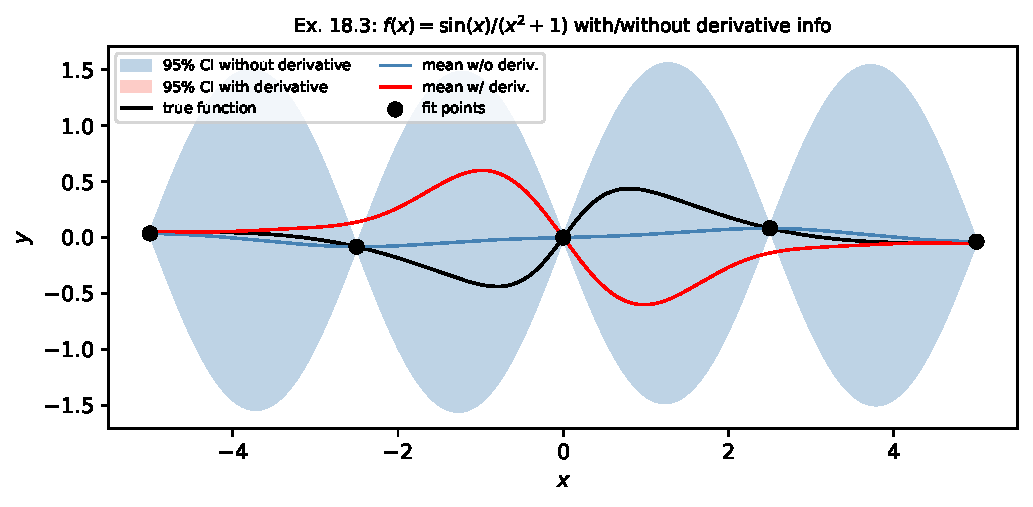
\includegraphics[width=\textwidth]{fig_exercise3.pdf}
        \caption{With derivative info (salmon), confidence interval is
                 tighter. Max.\ std with derivative $\approx 0.377$ at
                 $x\approx\pm3.8$. At least 8 points needed without
                 derivatives to match this accuracy.}
      \end{figure}
    \end{column}
  \end{columns}
\end{frame}

\begin{frame}{Exercise 18.10 -- Kernel Selection via Cross-Validation}
  \begin{columns}[T]
    \begin{column}{0.55\textwidth}
      \textbf{Problem:} Select best kernel for data
      $\{(1,0),(2,-1),(3,-2),(4,1),(5,0)\}$ using leave-one-out (LOO)
      cross-validation.\\
      \vspace{0.4em}
      Maximise the sum of LOO log-likelihoods across all folds.\\
      \vspace{0.3em}
      \textbf{Results:}
      \begin{center}
        \renewcommand{\arraystretch}{1.2}
        \begin{tabular}{lc}
          \toprule
          \textbf{Kernel} & \textbf{Log-lik.}\\
          \midrule
          $\exp(-\|x-x'\|)$         & $-8.688$\\
          $\exp(-\|x-x'\|^2)$       & $-9.010$\\
          $(1+\|x-x'\|)^{-1}$       & $-9.579$\\
          $(1+\|x-x'\|^2)^{-1}$     & $-10.195$\\
          $(1+\|x-x'\|)^{-2}$       & $\mathbf{-8.088}$ \\
          \bottomrule
        \end{tabular}
      \end{center}
      \textbf{Best:} Rational quadratic $(1+\|x-x'\|)^{-2}$.
    \end{column}
    \begin{column}{0.42\textwidth}
      \textbf{LOO CV procedure:}
      \begin{enumerate}
        \item For each fold $i$ ($i=1\ldots 5$):
          \begin{itemize}
            \item Hold out point $(x_i, y_i)$
            \item Fit GP on remaining 4 points
            \item Evaluate $\log p(y_i \mid x_i, \text{other data})$
          \end{itemize}
        \item Sum log-likelihoods over folds
        \item Select kernel with highest total
      \end{enumerate}
      \vspace{0.5em}
      \textbf{Key insight:} LOO-CV is a principled model selection
      criterion that avoids overfitting to the training set.
    \end{column}
  \end{columns}
\end{frame}

\begin{frame}[allowframebreaks]{Key Takeaways}
  \begin{block}{Gaussian Distribution (Sec.\ 18.1)}
    \begin{itemize}
      \item $n$-dimensional Gaussian parametrised by $\bmu$ and $\bSigma$
      \item Marginal: retain a subset of variables -- still Gaussian
      \item Conditional: condition on some variables -- still Gaussian
      \item Closed-form formulas for both are the engine of GP inference
    \end{itemize}
  \end{block}

  \begin{block}{Gaussian Processes (Sec.\ 18.2)}
    \begin{itemize}
      \item Distribution over functions, defined by mean function $m(\bx)$
            and kernel function $k(\bx,\bx')$
      \item Kernel choice controls smoothness of function samples
      \item Nonparametric: model complexity grows with data
    \end{itemize}
  \end{block}

  \begin{block}{Prediction (Sec.\ 18.3)}
    \begin{itemize}
      \item Posterior mean and variance at query points computed analytically
      \item Uncertainty grows far from training data, approaches prior far away
      \item Prediction cost $O(m^3)$; dominant cost is matrix inversion
    \end{itemize}
  \end{block}

  \framebreak

  \begin{block}{Gradient Measurements (Sec.\ 18.4)}
    \begin{itemize}
      \item Derivative observations seamlessly incorporated via derived kernels
      \item Gradient covariance functions derived by differentiating the kernel
      \item Each gradient observation adds $n$ constraints --- powerful when
            gradients are cheap
    \end{itemize}
  \end{block}

  \begin{block}{Noisy Measurements (Sec.\ 18.5)}
    \begin{itemize}
      \item Model noise as $y = f(\bx) + z$, $z\sim\Norm(0,\nu)$
      \item Equivalent to adding $\nu\mathbf{I}$ to training kernel matrix
      \item Posterior no longer interpolates --- smooths through noisy data
    \end{itemize}
  \end{block}

  \begin{block}{Fitting GPs (Sec.\ 18.6)}
    \begin{itemize}
      \item Maximise log marginal likelihood to learn kernel hyperparameters
      \item Balances data fit vs.\ model complexity (Bayesian Occam's razor)
      \item Use gradient-based optimisation (L-BFGS-B) with multiple restarts
      \item Can also use leave-one-out cross-validation for kernel selection
    \end{itemize}
  \end{block}
\end{frame}

% ══════════════════════════════════════════════════════════════════════════════
\begin{frame}{Further Reading}
  \begin{columns}[T]
    \begin{column}{0.55\textwidth}
      \textbf{Textbook:}
      \begin{itemize}
        \item Rasmussen \& Williams, \emph{Gaussian Processes for Machine
              Learning}, MIT Press, 2006 (freely available online)
        \item Kochenderfer \& Wheeler, \emph{Algorithms for Optimization},
              2nd ed., MIT Press, 2026
      \end{itemize}
      \vspace{0.4em}
      \textbf{Libraries (Python):}
      \begin{itemize}
        \item \texttt{scikit-learn}: \texttt{GaussianProcessRegressor}
        \item \texttt{GPy}: full-featured GP library
        \item \texttt{GPyTorch}: GPU-accelerated GPs (PyTorch)
        \item \texttt{BoTorch}: Bayesian optimisation with GPs
      \end{itemize}
    \end{column}
    \begin{column}{0.42\textwidth}
      \textbf{Next chapter:}\\
      Chapter 19 -- Surrogate Optimisation\\
      (Bayesian optimisation using GP posteriors)
      \vspace{0.5em}
      \begin{itemize}
        \item Acquisition functions (EI, UCB, PI)
        \item Exploration vs.\ exploitation trade-off
        \item Optimising the acquisition function
      \end{itemize}
    \end{column}
  \end{columns}
\end{frame}

\end{document}
